\section{Intérieur, adhérent, frontière}
\subsection{Intérieur}
\begin{definition}
    Soit $A \subset E$.
    \begin{enumerate}
        \item $x_0 \in E$ est intérieur à $A$ si  $\exists \, \delta > 0$ tel que:
            \[
            B(x_0, \delta) \subset A
            \] 
        \item $Int(A)$ (intérieur de A) = tous les points intériers à  $A$. (aussi noté $A$)
    \end{enumerate}
\end{definition}
\begin{intuition}
   $Int(A)$ est un ensemble qui se trouve totallement dans $A$ et qui est loin des bords de  $A$.
\end{intuition}
\begin{figure}[ht]
    \centering
    \incfig{interieur-exemple}
    \caption{Exemple d'un intérieur}
    \label{fig:interieur-exemple}
\end{figure}
\begin{prop}
   $Int(A)$ est le plus grand ouvert inclus dans  $A$. De manière équivalente, $Int(A)$ est la réunion de tous les ouverts inclus dans  $A$.
\end{prop}
\begin{preuve}
   \begin{enumerate}
       \item $Int(A) \subset A$: clair
       \item \underline{$Int(A)$ est ouvert:} \\
           Soit $x_0 \in Int(A)$. 
           \par
           \textbf{But:} trouver $\delta_0$ tel que  $B(x_0, \delta_0) \subset Int(A)$. Trouver $\delta_0$ tel que si $d(x_0, x) < \delta_0$ alors $x \in Int(A)$ ?
           \par
           \textbf{Hyp:}  $x_0 \in Int(A)$. $\exists \delta_1 > 0$ tel que $B(x_0, \delta_1) \subset A$. On a vu que $B(x_0, \delta_1)$ est ouvert.
           Je dis que $B(x_0, \delta_1) \subset Int(A)$.
           \par
           \textbf{Preuve}: Soit $x \in B(x_0, \delta_1)$. $B(x_0, \delta_1)$ ouvert, donc $\exists \delta_2 > 0$ tel que $B(x, \delta_2) \subset B(x_0, \delta_1) \subset A$. Donc $x \in Int(A)$, donc  $B(x_0, \delta_1) \subset Int(A)$.\par
           $Int(A)$ est ouvert.
       \item Si $U$ est ouvert et  $U \subset A$ alors $U \subset Int(A)$?
           \par
           $x_0 \in U$. $U$ ouvert  $\implies$ $\exists \delta$ tel que $B(x_0, \delta) \subset U \subset A$ $\implies$ $x_0 \in Int(A)$
   \end{enumerate} 
\end{preuve}

\subsection{Adhérent}
\begin{definition}
    Soit $A \subset E$. 
    \begin{enumerate}
        \item $x_0 \in E$ est \underline{adhérent} à $A$, si  $\forall \delta > 0, \, B(x_0, \delta)$ intérsecte $A$. (équivalent à $d(x_0, A) = 0$)
        \item $Adh(A)$ (adhérence ou fermeture de $A$) = ensemble des points adhérents à $A$ (aussi noté $\overline{A}$)
    \end{enumerate}
\end{definition}
\begin{intuition}
   Adherent aide à completer des ensembles. Si $A$ est ouvert, alors ses bords n'appartiennent pas à  $A$, mais ils appartiennent à  $Adh(A)$ .
\end{intuition}
\begin{figure}[H]
   \centering 
    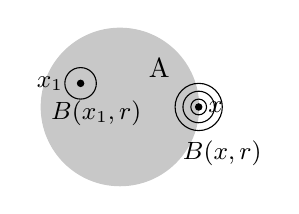
\begin{tikzpicture}
            \definecolor{lightgray}{RGB}{200, 200, 200}
        \filldraw[color=lightgray] (0,0) circle (1cm); 
        \coordinate (x) at (1, 0);
        \filldraw[color=black] (x) circle (0.4mm);
        \node[right] (_) at (x){\small $x$};
        \node (_) at (0.5, 0.5){A};

        \draw (x) circle (0.2cm);
        \draw (x) circle (0.3cm);
        \draw (x) circle (0.1cm);
        \node[below] (_) at (1.3, -0.3){\small $B(x, r)$};

        \draw (-0.5, 0.3) circle (0.2cm);
        \filldraw[color=black] (-0.5, 0.3) circle (0.4mm);
        \node[left](_) at (-0.6, 0.3){\small $x_1$};
        \node[below] (_) at (-0.3, 0.2){\small $B(x_1, r)$};
    \end{tikzpicture} 
    \caption{Adhérent}
\end{figure}
\begin{prop}
   $Adh(A)$ est le plus petit fermé qui contient $A$ (l'intérsection de tous les fermés qui contiennent $A$)
\end{prop}
\begin{preuve}
   \begin{enumerate}
       \item $A \subset Adh(A)$ clair
       \item $Adh(A)$ est fermé?
           \par On montre que  $E \setminus Adh(A)$ est ouvert. \par 
           $x_0 \in Adh(A)$ $\iff$ $\forall \delta > 0, \, B(x_0, \delta) \cap A \neq \O$ \par
           $x_0 \not\in Adh(A)$ $\iff$ $\exists \delta_0 > 0$ tq $B(x_0, \delta_0) \cap A = \O$ $\iff$ $\exists \delta_0>0$ tq $B(x_0, \delta_0) \subset E\setminus A$ $\iff$ $x_0 \in Int(E\setminus A)$ 
           \par Alors:
           \begin{align*}
               &E \setminus Adh(A) = Int(E \setminus A)\\
               &Adh(A) = (Int(\underbrace{A^{c}}_{= E \setminus A}))^{c}
           \end{align*}
   \end{enumerate} 
\end{preuve}
\begin{definition}
    Soit $A \subset B$. On dit que $A$ est dense dans  $B$ si  $B \subset Adh(A)$
    \par
    Soit $x_0 \in B, \, \forall \epsilon > 0 \, \exists  x_{\epsilon} \in A$ tel que $d(x_0, x_{\epsilon}) < \epsilon$
\end{definition}
\begin{eg}
   \[
       \Q^2 = \{(x, y): x,y \in \Q\} \text{ dense dans } \R^2
   \]  
   
\end{eg}

\subsection{Frontière}
 \begin{definition}
     Soit $A \subset E$. La \textbf{frontière} de $A$ (ou le bord de $A$) noté $Fr(A)$ ou  $\partial A$ c'est:
      \[
     Adh(A) \cap Adh(E \setminus A)
     \] 
 \end{definition}
 \begin{eg} dans $\R$
    \begin{enumerate}
        \item $Int(\Q) = \O$
        \item $Int(\R \setminus \Q) = \O$
        \item $Adh(\Q) = \R$
        \item $Adh(\R \setminus \Q) = \R$
        \item $Fr(\Q) = \R$
        \item $Fr(\R \setminus \Q) = \R$
    \end{enumerate} 
 \end{eg}
 \begin{eg} $E = \{a, b, c\}$
    On pose:
    \begin{itemize}
        \item $d(a,a) = d(b,b) = d(c,c) = 0$
        \item  $d(a,b) = d(b,a) = d(b,c) = d(b,c) = 1$
        \item  $d(a,c) = d(c, a) = 2$
    \end{itemize}
    \[
        B(a,2) = \{a, b\} = Adh(B(a, 2))
    \] 
    \[
        B_f(a, 2) = \{a, b, c\}
    \] 
 \end{eg}
 \begin{prop}
    \begin{enumerate}
        \item $Int(A) \subset A \subset Adh(A)$
        \item $E = Int(E \setminus A) \cup Fr(A) \cup Int(A)$ (union disjointe)
        \item $E \setminus Int(A) = Adh(E \setminus A)$
        \item $E \setminus Adh(A) = Int(E \setminus A)$
        \item $Fr(A) = Adh(A) \setminus Int(A)$
    \end{enumerate} 
 \end{prop}
 \begin{prop}
     \begin{enumerate}
         \item $A$ ouvert  $\iff$ $A = Int(A)$
         \item  $A$ fermé  $\iff$ $A = Adh(A)$
         \item  $x \in Adh(A)$  $\iff$ $d(x, A) = 0$
         \item  $x \in Int(A)$  $\iff$ $d(x, E \setminus A) > 0$
     \end{enumerate}
 \end{prop}

 \section{Suite dans un éspace métrique}
 \begin{definition}
     $E$ un ensemble. Une suite dans $E$: notée $(u_n)_{n \in \N}$ c'est une fonction $u:  \N \to E$ où $u(n)$ est noté  $u_n$ est le le  $\text{n}^{\text{ième}}$ terme de la suite $(u_n)_{n \in \N}$.
     \par
     Si $E = \R^d$
     \[
     \R^d \ni X_n = (x_{1,n}, \ldots, x_{d,n})
     \] 
 où $(x_{i,n})_{n \in \N}$ suites dans $\R$
 \end{definition}
 \begin{definition}
     Soit $(x_n)$ une suite dans  $E$ et  $x \in E$. On dit que  $\lim_{n \to \infty} x_n = x$ si $\lim_{n \to \infty} d(x_n, x) = 0$.
     \par
     ($\forall \epsilon > 0, \, \exists N \in \N \, \text{ tq si } n \ge N, \, d(x_n, x) < \epsilon$)
 \end{definition}
 \begin{prop}
     $(x_n)_{n \in \N}$ est bornée si $\{x_n : n \in \N\} (\subset E)$ est un ensemble borné. 
 \end{prop}
 \begin{remark}
    dans $\R^d$ muni de $d_2$ (distance euclidienne)

    \begin{align*}
        &X_n = (x_{1,n}, \ldots, x_{d,n})\\
        &X = (x_1, \ldots, x_d)
    \end{align*}
    \[
    \lim_{n \to \infty} X_n = X \iff \lim_{n \to \infty} x_{i,n} = x_i \quad (1 \le i \le d)
    \] 
 \end{remark}
 \begin{prop}
    la limite d'une suite convergente est unique. 
 \end{prop}
 \begin{preuve}
    \[
    \text{Si } X_n \xrightarrow[n \to \infty]{} X \text{ et } X_n \xrightarrow[n \to \infty]{} X'
    \]  
    \[
        d(X, X') \le \underbrace{d(X, X_n)}_{\to 0} + \underbrace{d(X_n, X')}_{\to 0} \implies d(X, X') = 0 \implies X = X'
    \] 
 \end{preuve}
 \begin{prop}\label{prop:suite-lien-avec-adherence}
     (lien aven l'adhérence) 
     \begin{enumerate}
         \item $x \in Adh(A)$ si et seulement s'il existe une suite  $(x_n)$ d'éléments de  $A$ telle que  $\lim_{n \to \infty} x_n = x$
         \item $A$ est fermé ssi pour toute suite  $(x_n)$ d'éléments de  $A$ qui converge vers $x \in E$ on a $x \in A$
     \end{enumerate}
 \end{prop}
\begin{intuition}
   \begin{enumerate}
       \item Si $(x_n)_{n \in \N}$ est d'éléments de  $A$ ($\forall n \in N, \, x_n \in A$), donc elle converge vers un éléments $x$ qui peut être soit dans  $A$, soit à la borne des éléments de  $A$, alors à la frontière. 
       \item Si la limite de toute suite $(x_n)_{n \in \N}$ des éléments de  $A$ est aussi dans  $A$, alors la frontière de  $A$ est inclu dans  $A$. Car l'une des suites tend vers la borne.
   \end{enumerate} 
\end{intuition}
\begin{preuve} de Prop. \ref{prop:suite-lien-avec-adherence}
    \begin{enumerate}
        \item ($\impliedby$) Soit $(x_n)$ avec  $x_n \in A \quad \forall n \in \N$ et $\lim_{n \to \infty} x_n = x$.
            \par
            J'ai $d(x_n, x) \xrightarrow[n \to \infty]{} 0$ et $x_n \in A$, donc
             \[
                 inf_{y \in A}(d(x, y)) = 0 = d(x, A)
            \] 
            \[
            d(x, A) = 0 \iff x \in Adh(A)
            \] 
            \par
            ($\implies$) Soit $x \in Adh(A)$
             \begin{align*}
                 \iff& d(x, A) = 0\\
                \iff& \forall \epsilon > 0, \, \exists x_{\epsilon} \in A \text{ tel que } d(x, x_{\epsilon}) < \epsilon
            \end{align*}
            Prendre $\epsilon = \frac{1}{n}$, je pose $u_n = x_{\frac{1}{n}}$. $u_n \in A$  $d(x, u_n) < \frac{1}{n}$, donc $\lim_{n \to \infty} u_n = x$ 
        \item ($\implies$) Soit $A$ fermé, donc 
             \[
            A = Adh(A)
            \] 
            Si $(x_n)$ suite dans  $A$ qui converge vers  $x$.
             \[
            x \in Adh(A) = A
            \] 
            ($\impliedby$) On dit que $Adh(A) \subset A$. Comme $A \subset Adh(A)$, donc $A = Adh(A)$
    \end{enumerate} 
 \end{preuve}
